% Options for packages loaded elsewhere
\PassOptionsToPackage{unicode}{hyperref}
\PassOptionsToPackage{hyphens}{url}
%
\documentclass[
]{article}
\usepackage{amsmath,amssymb}
\usepackage{lmodern}
\usepackage{iftex}
\ifPDFTeX
  \usepackage[T1]{fontenc}
  \usepackage[utf8]{inputenc}
  \usepackage{textcomp} % provide euro and other symbols
\else % if luatex or xetex
  \usepackage{unicode-math}
  \defaultfontfeatures{Scale=MatchLowercase}
  \defaultfontfeatures[\rmfamily]{Ligatures=TeX,Scale=1}
\fi
% Use upquote if available, for straight quotes in verbatim environments
\IfFileExists{upquote.sty}{\usepackage{upquote}}{}
\IfFileExists{microtype.sty}{% use microtype if available
  \usepackage[]{microtype}
  \UseMicrotypeSet[protrusion]{basicmath} % disable protrusion for tt fonts
}{}
\makeatletter
\@ifundefined{KOMAClassName}{% if non-KOMA class
  \IfFileExists{parskip.sty}{%
    \usepackage{parskip}
  }{% else
    \setlength{\parindent}{0pt}
    \setlength{\parskip}{6pt plus 2pt minus 1pt}}
}{% if KOMA class
  \KOMAoptions{parskip=half}}
\makeatother
\usepackage{xcolor}
\usepackage[margin=1in]{geometry}
\usepackage{color}
\usepackage{fancyvrb}
\newcommand{\VerbBar}{|}
\newcommand{\VERB}{\Verb[commandchars=\\\{\}]}
\DefineVerbatimEnvironment{Highlighting}{Verbatim}{commandchars=\\\{\}}
% Add ',fontsize=\small' for more characters per line
\usepackage{framed}
\definecolor{shadecolor}{RGB}{248,248,248}
\newenvironment{Shaded}{\begin{snugshade}}{\end{snugshade}}
\newcommand{\AlertTok}[1]{\textcolor[rgb]{0.94,0.16,0.16}{#1}}
\newcommand{\AnnotationTok}[1]{\textcolor[rgb]{0.56,0.35,0.01}{\textbf{\textit{#1}}}}
\newcommand{\AttributeTok}[1]{\textcolor[rgb]{0.77,0.63,0.00}{#1}}
\newcommand{\BaseNTok}[1]{\textcolor[rgb]{0.00,0.00,0.81}{#1}}
\newcommand{\BuiltInTok}[1]{#1}
\newcommand{\CharTok}[1]{\textcolor[rgb]{0.31,0.60,0.02}{#1}}
\newcommand{\CommentTok}[1]{\textcolor[rgb]{0.56,0.35,0.01}{\textit{#1}}}
\newcommand{\CommentVarTok}[1]{\textcolor[rgb]{0.56,0.35,0.01}{\textbf{\textit{#1}}}}
\newcommand{\ConstantTok}[1]{\textcolor[rgb]{0.00,0.00,0.00}{#1}}
\newcommand{\ControlFlowTok}[1]{\textcolor[rgb]{0.13,0.29,0.53}{\textbf{#1}}}
\newcommand{\DataTypeTok}[1]{\textcolor[rgb]{0.13,0.29,0.53}{#1}}
\newcommand{\DecValTok}[1]{\textcolor[rgb]{0.00,0.00,0.81}{#1}}
\newcommand{\DocumentationTok}[1]{\textcolor[rgb]{0.56,0.35,0.01}{\textbf{\textit{#1}}}}
\newcommand{\ErrorTok}[1]{\textcolor[rgb]{0.64,0.00,0.00}{\textbf{#1}}}
\newcommand{\ExtensionTok}[1]{#1}
\newcommand{\FloatTok}[1]{\textcolor[rgb]{0.00,0.00,0.81}{#1}}
\newcommand{\FunctionTok}[1]{\textcolor[rgb]{0.00,0.00,0.00}{#1}}
\newcommand{\ImportTok}[1]{#1}
\newcommand{\InformationTok}[1]{\textcolor[rgb]{0.56,0.35,0.01}{\textbf{\textit{#1}}}}
\newcommand{\KeywordTok}[1]{\textcolor[rgb]{0.13,0.29,0.53}{\textbf{#1}}}
\newcommand{\NormalTok}[1]{#1}
\newcommand{\OperatorTok}[1]{\textcolor[rgb]{0.81,0.36,0.00}{\textbf{#1}}}
\newcommand{\OtherTok}[1]{\textcolor[rgb]{0.56,0.35,0.01}{#1}}
\newcommand{\PreprocessorTok}[1]{\textcolor[rgb]{0.56,0.35,0.01}{\textit{#1}}}
\newcommand{\RegionMarkerTok}[1]{#1}
\newcommand{\SpecialCharTok}[1]{\textcolor[rgb]{0.00,0.00,0.00}{#1}}
\newcommand{\SpecialStringTok}[1]{\textcolor[rgb]{0.31,0.60,0.02}{#1}}
\newcommand{\StringTok}[1]{\textcolor[rgb]{0.31,0.60,0.02}{#1}}
\newcommand{\VariableTok}[1]{\textcolor[rgb]{0.00,0.00,0.00}{#1}}
\newcommand{\VerbatimStringTok}[1]{\textcolor[rgb]{0.31,0.60,0.02}{#1}}
\newcommand{\WarningTok}[1]{\textcolor[rgb]{0.56,0.35,0.01}{\textbf{\textit{#1}}}}
\usepackage{graphicx}
\makeatletter
\def\maxwidth{\ifdim\Gin@nat@width>\linewidth\linewidth\else\Gin@nat@width\fi}
\def\maxheight{\ifdim\Gin@nat@height>\textheight\textheight\else\Gin@nat@height\fi}
\makeatother
% Scale images if necessary, so that they will not overflow the page
% margins by default, and it is still possible to overwrite the defaults
% using explicit options in \includegraphics[width, height, ...]{}
\setkeys{Gin}{width=\maxwidth,height=\maxheight,keepaspectratio}
% Set default figure placement to htbp
\makeatletter
\def\fps@figure{htbp}
\makeatother
\setlength{\emergencystretch}{3em} % prevent overfull lines
\providecommand{\tightlist}{%
  \setlength{\itemsep}{0pt}\setlength{\parskip}{0pt}}
\setcounter{secnumdepth}{-\maxdimen} % remove section numbering
\ifLuaTeX
  \usepackage{selnolig}  % disable illegal ligatures
\fi
\IfFileExists{bookmark.sty}{\usepackage{bookmark}}{\usepackage{hyperref}}
\IfFileExists{xurl.sty}{\usepackage{xurl}}{} % add URL line breaks if available
\urlstyle{same} % disable monospaced font for URLs
\hypersetup{
  pdftitle={2. Fish Classifier},
  pdfauthor={Justin König},
  hidelinks,
  pdfcreator={LaTeX via pandoc}}

\title{2. Fish Classifier}
\author{Justin König}
\date{08.05.2023}

\begin{document}
\maketitle

{
\setcounter{tocdepth}{2}
\tableofcontents
}
\begin{Shaded}
\begin{Highlighting}[]
\CommentTok{\# load data frame}
\NormalTok{fish\_df }\OtherTok{\textless{}{-}} \FunctionTok{read.csv2}\NormalTok{(}\StringTok{"fishcatch.csv"}\NormalTok{)}

\CommentTok{\# remove unnecessary data}
\NormalTok{fish\_df }\OtherTok{\textless{}{-}}\NormalTok{ fish\_df[}\DecValTok{48}\SpecialCharTok{:}\FunctionTok{nrow}\NormalTok{(fish\_df),]}

\FunctionTok{colnames}\NormalTok{(fish\_df) }\OtherTok{\textless{}{-}} \FunctionTok{c}\NormalTok{(}\StringTok{"Species"}\NormalTok{, }\StringTok{"Length1"}\NormalTok{, }\StringTok{"Length2"}\NormalTok{, }\StringTok{"Length3"}\NormalTok{,}\StringTok{"Height"}\NormalTok{, }\StringTok{"Width"}\NormalTok{,}
                       \StringTok{"sex"}\NormalTok{, }\StringTok{"Weight"}\NormalTok{)}

\NormalTok{fish\_df }\OtherTok{\textless{}{-}} \FunctionTok{as.data.frame}\NormalTok{(}\FunctionTok{apply}\NormalTok{(fish\_df, }\DecValTok{2}\NormalTok{, }\ControlFlowTok{function}\NormalTok{(x) }\FunctionTok{gsub}\NormalTok{(}\StringTok{","}\NormalTok{, }\StringTok{"."}\NormalTok{, x)))}

\CommentTok{\# List the columns you want to convert to numeric}
\NormalTok{columns\_to\_convert }\OtherTok{\textless{}{-}} \FunctionTok{c}\NormalTok{(}\StringTok{"Length1"}\NormalTok{, }\StringTok{"Length2"}\NormalTok{, }\StringTok{"Length3"}\NormalTok{,}\StringTok{"Height"}\NormalTok{, }\StringTok{"Width"}\NormalTok{,}
                       \StringTok{"Weight"}\NormalTok{)}

\CommentTok{\# counts fish classes}
\NormalTok{fish\_count }\OtherTok{\textless{}{-}}\NormalTok{ fish\_df }\SpecialCharTok{\%\textgreater{}\%}
  \FunctionTok{group\_by}\NormalTok{(Species) }\SpecialCharTok{\%\textgreater{}\%}
  \FunctionTok{summarise}\NormalTok{(}\AttributeTok{Count =} \FunctionTok{n}\NormalTok{())}

\CommentTok{\# Convert the specified columns to numeric}
\NormalTok{fish\_df }\OtherTok{\textless{}{-}}\NormalTok{ fish\_df }\SpecialCharTok{\%\textgreater{}\%}
  \FunctionTok{mutate}\NormalTok{(}\FunctionTok{across}\NormalTok{(}\FunctionTok{all\_of}\NormalTok{(columns\_to\_convert), as.numeric))}


\NormalTok{train\_data }\OtherTok{\textless{}{-}}\NormalTok{ fish\_df[}\SpecialCharTok{!}\NormalTok{(}\FunctionTok{seq\_len}\NormalTok{(}\FunctionTok{nrow}\NormalTok{(fish\_df)) }\SpecialCharTok{\%\%} \DecValTok{10} \SpecialCharTok{==} \DecValTok{0}\NormalTok{), ]}

\CommentTok{\# Testdatensatz erstellen (jeder 10. Fisch)}
\NormalTok{test\_data }\OtherTok{\textless{}{-}}\NormalTok{ fish\_df[}\FunctionTok{seq}\NormalTok{(}\DecValTok{1}\NormalTok{, }\FunctionTok{nrow}\NormalTok{(fish\_df), }\AttributeTok{by =} \DecValTok{10}\NormalTok{), ]}
\end{Highlighting}
\end{Shaded}

\begin{Shaded}
\begin{Highlighting}[]
\FunctionTok{ggplot}\NormalTok{(fish\_count, }\FunctionTok{aes}\NormalTok{(}\AttributeTok{x =}\NormalTok{ Species, }\AttributeTok{y =}\NormalTok{ Count)) }\SpecialCharTok{+}
  \FunctionTok{geom\_bar}\NormalTok{(}\AttributeTok{stat =} \StringTok{"identity"}\NormalTok{, }\AttributeTok{fill =} \StringTok{"steelblue"}\NormalTok{) }\SpecialCharTok{+}
  \FunctionTok{theme\_classic}\NormalTok{() }\SpecialCharTok{+}
  \FunctionTok{labs}\NormalTok{(}\AttributeTok{title =} \StringTok{"Fish Count per Species"}\NormalTok{,}
       \AttributeTok{x =} \StringTok{"Species"}\NormalTok{,}
       \AttributeTok{y =} \StringTok{"Count"}\NormalTok{)}
\end{Highlighting}
\end{Shaded}

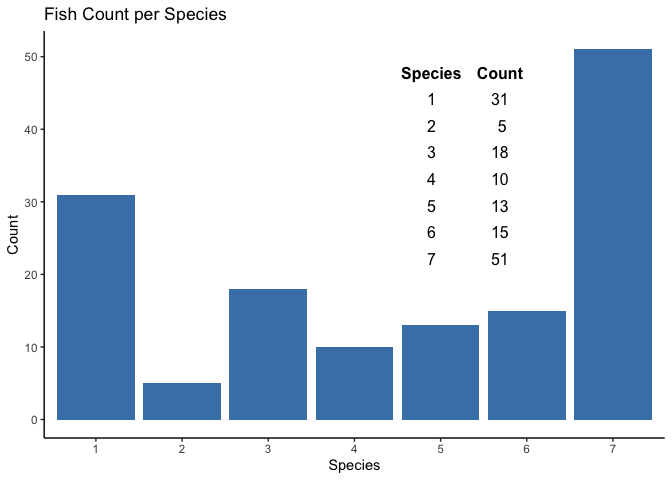
\includegraphics{Fish-Classifier_files/figure-latex/visualitation-1.pdf}

\begin{Shaded}
\begin{Highlighting}[]
\CommentTok{\# Specify the fish species you are interested in}
\NormalTok{fish\_species }\OtherTok{\textless{}{-}} \FunctionTok{c}\NormalTok{(}\StringTok{"1"}\NormalTok{)}

\CommentTok{\# Calculate the mean for the specified fish species}
\NormalTok{mean\_species }\OtherTok{\textless{}{-}}\NormalTok{ fish\_df }\SpecialCharTok{\%\textgreater{}\%}
  \FunctionTok{filter}\NormalTok{(Species }\SpecialCharTok{==}\NormalTok{ fish\_species) }\SpecialCharTok{\%\textgreater{}\%}
  \FunctionTok{summarise}\NormalTok{(}\AttributeTok{Mean\_Length1 =} \FunctionTok{mean}\NormalTok{(Length1, }\AttributeTok{na.rm =} \ConstantTok{TRUE}\NormalTok{),}
            \AttributeTok{Mean\_Length2 =} \FunctionTok{mean}\NormalTok{(Length2, }\AttributeTok{na.rm =} \ConstantTok{TRUE}\NormalTok{),}
            \AttributeTok{Mean\_Length3 =} \FunctionTok{mean}\NormalTok{(Length3, }\AttributeTok{na.rm =} \ConstantTok{TRUE}\NormalTok{),}
            \AttributeTok{Mean\_Height =} \FunctionTok{mean}\NormalTok{(Height, }\AttributeTok{na.rm =} \ConstantTok{TRUE}\NormalTok{),}
            \AttributeTok{Mean\_Width =} \FunctionTok{mean}\NormalTok{(Width, }\AttributeTok{na.rm =} \ConstantTok{TRUE}\NormalTok{),}
            \AttributeTok{Mean\_Weight =} \FunctionTok{mean}\NormalTok{(Weight, }\AttributeTok{na.rm =} \ConstantTok{TRUE}\NormalTok{))}

\CommentTok{\# Print the mean values}
\FunctionTok{print}\NormalTok{(mean\_species)}
\end{Highlighting}
\end{Shaded}

\begin{verbatim}
##   Mean_Length1 Mean_Length2 Mean_Length3 Mean_Height Mean_Width Mean_Weight
## 1     30.32941     33.14118     38.38529    39.59118   14.14706         626
\end{verbatim}

\begin{Shaded}
\begin{Highlighting}[]
\CommentTok{\# Load the data}
\NormalTok{df }\OtherTok{\textless{}{-}}\NormalTok{ fish\_df}

\CommentTok{\# Split the data into training and testing sets}
\FunctionTok{set.seed}\NormalTok{(}\DecValTok{42}\NormalTok{)}
\NormalTok{split\_index }\OtherTok{\textless{}{-}} \FunctionTok{sample}\NormalTok{(}\DecValTok{1}\SpecialCharTok{:}\FunctionTok{nrow}\NormalTok{(fish\_df), }\FloatTok{0.7} \SpecialCharTok{*} \FunctionTok{nrow}\NormalTok{(fish\_df))}
\NormalTok{train\_data }\OtherTok{\textless{}{-}}\NormalTok{ fish\_df[split\_index, ]}
\NormalTok{test\_data }\OtherTok{\textless{}{-}}\NormalTok{ fish\_df[}\SpecialCharTok{{-}}\NormalTok{split\_index, ]}

\CommentTok{\# Calculate the mean, covariance, and a{-}priori probability for each fish species}
\NormalTok{species\_list }\OtherTok{\textless{}{-}} \FunctionTok{unique}\NormalTok{(train\_data}\SpecialCharTok{$}\NormalTok{Species)}
\NormalTok{stats\_list }\OtherTok{\textless{}{-}} \FunctionTok{lapply}\NormalTok{(species\_list, }\ControlFlowTok{function}\NormalTok{(species) \{}
\NormalTok{  species\_data }\OtherTok{\textless{}{-}}\NormalTok{ train\_data[train\_data}\SpecialCharTok{$}\NormalTok{Species }\SpecialCharTok{==}\NormalTok{ species, }\FunctionTok{c}\NormalTok{(}\StringTok{"Length1"}\NormalTok{, }\StringTok{"Length2"}\NormalTok{, }\StringTok{"Length3"}\NormalTok{, }\StringTok{"Height"}\NormalTok{, }\StringTok{"Width"}\NormalTok{)]}
\NormalTok{  n }\OtherTok{\textless{}{-}} \FunctionTok{nrow}\NormalTok{(species\_data)}
  
  \FunctionTok{list}\NormalTok{(}\AttributeTok{mean =} \FunctionTok{colMeans}\NormalTok{(species\_data),}
       \AttributeTok{cov =} \FunctionTok{cov}\NormalTok{(species\_data) }\SpecialCharTok{+} \FunctionTok{diag}\NormalTok{(}\FloatTok{1e{-}6}\NormalTok{, }\FunctionTok{ncol}\NormalTok{(species\_data)),}
       \AttributeTok{prior =}\NormalTok{ n }\SpecialCharTok{/} \FunctionTok{nrow}\NormalTok{(train\_data))}
\NormalTok{\})}

\FunctionTok{names}\NormalTok{(stats\_list) }\OtherTok{\textless{}{-}}\NormalTok{ species\_list}

\CommentTok{\# Multivariate Gaussian density function}
\NormalTok{multivariate\_gaussian }\OtherTok{\textless{}{-}} \ControlFlowTok{function}\NormalTok{(x, mean, cov) \{}
\NormalTok{  k }\OtherTok{\textless{}{-}} \FunctionTok{length}\NormalTok{(mean)}
  \FunctionTok{exp}\NormalTok{(}\SpecialCharTok{{-}}\FloatTok{0.5} \SpecialCharTok{*} \FunctionTok{t}\NormalTok{(x }\SpecialCharTok{{-}}\NormalTok{ mean) }\SpecialCharTok{\%*\%} \FunctionTok{solve}\NormalTok{(cov, x }\SpecialCharTok{{-}}\NormalTok{ mean)) }\SpecialCharTok{/} \FunctionTok{sqrt}\NormalTok{((}\DecValTok{2} \SpecialCharTok{*}\NormalTok{ pi)}\SpecialCharTok{\^{}}\NormalTok{k }\SpecialCharTok{*} \FunctionTok{det}\NormalTok{(cov))}
\NormalTok{\}}

\CommentTok{\# QDA classifier}
\NormalTok{classify\_fish\_qda }\OtherTok{\textless{}{-}} \ControlFlowTok{function}\NormalTok{(lengths) \{}
\NormalTok{  likelihoods }\OtherTok{\textless{}{-}} \FunctionTok{sapply}\NormalTok{(stats\_list, }\ControlFlowTok{function}\NormalTok{(params) \{}
\NormalTok{    likelihood }\OtherTok{\textless{}{-}} \FunctionTok{multivariate\_gaussian}\NormalTok{(lengths, params}\SpecialCharTok{$}\NormalTok{mean, params}\SpecialCharTok{$}\NormalTok{cov)}
\NormalTok{    likelihood }\SpecialCharTok{*}\NormalTok{ params}\SpecialCharTok{$}\NormalTok{prior}
\NormalTok{  \})}
  
  \FunctionTok{names}\NormalTok{(likelihoods)[}\FunctionTok{which.max}\NormalTok{(likelihoods)]}
\NormalTok{\}}

\CommentTok{\# Classify each fish in the test set}
\NormalTok{predicted\_species }\OtherTok{\textless{}{-}} \FunctionTok{apply}\NormalTok{(test\_data[, }\FunctionTok{c}\NormalTok{(}\StringTok{"Length1"}\NormalTok{, }\StringTok{"Length2"}\NormalTok{, }\StringTok{"Length3"}\NormalTok{, }\StringTok{"Height"}\NormalTok{, }\StringTok{"Width"}\NormalTok{)], }\DecValTok{1}\NormalTok{, classify\_fish\_qda)}

\CommentTok{\# Calculate the accuracy}
\NormalTok{correct\_predictions }\OtherTok{\textless{}{-}} \FunctionTok{sum}\NormalTok{(predicted\_species }\SpecialCharTok{==}\NormalTok{ test\_data}\SpecialCharTok{$}\NormalTok{Species)}
\NormalTok{total\_predictions }\OtherTok{\textless{}{-}} \FunctionTok{length}\NormalTok{(predicted\_species)}

\NormalTok{accuracy }\OtherTok{\textless{}{-}}\NormalTok{ correct\_predictions }\SpecialCharTok{/}\NormalTok{ total\_predictions}
\FunctionTok{cat}\NormalTok{(}\StringTok{"The accuracy of the QDA classifier on the test set is:"}\NormalTok{, accuracy }\SpecialCharTok{*} \DecValTok{100}\NormalTok{, }\StringTok{"\%}\SpecialCharTok{\textbackslash{}n}\StringTok{"}\NormalTok{)}
\end{Highlighting}
\end{Shaded}

\begin{verbatim}
## The accuracy of the QDA classifier on the test set is: 81.25 %
\end{verbatim}

\end{document}
